\UseRawInputEncoding
\documentclass[12pt]{article}
\title{ECE C143A Homework 3}
\usepackage{subcaption}
\author{Lawrence Liu}
\usepackage{graphicx}
\usepackage{amsmath}
\usepackage{pdfpages}
\newcommand{\Laplace}{\mathscr{L}}
\setlength{\parskip}{\baselineskip}%
\setlength{\parindent}{0pt}%
\usepackage{xcolor}
\usepackage{listings}
\definecolor{backcolour}{rgb}{0.95,0.95,0.92}
\usepackage{amssymb}
\lstdefinestyle{mystyle}{
    backgroundcolor=\color{backcolour}}
\lstset{style=mystyle}

\begin{document}
\maketitle
\section*{Problem 1}
\subsection*{(a)}
\begin{align*}
    P(M(s)=m)&=\sum_{n=m}^{\infty}\binom{n}{m}(1-p)^mp^{n-m}\frac{(\lambda s)^n}{n!}e^{-\lambda s}\\
            &=\sum_{n=m}^{\infty}\frac{n!}{m!(n-m)!}(1-p)^mp^{n-m}\frac{(\lambda s)^n}{n!}e^{-\lambda s}\\
            &=e^{-\lambda s}\frac{(1-p)^m}{m!}\sum_{n=m}^{\infty}\frac{p^{n-m}}{(n-m)!}(\lambda s)^n\\
            &=e^{-\lambda s}\frac{(1-p)^m}{m!}(\lambda s)^{m}\sum_{n=m}^{\infty}\frac{p^{n-m}}{(n-m)!}(\lambda s)^{n-m}\\
            &=e^{-\lambda s}\frac{(1-p)^m}{m!}(\lambda s)^{m}\sum_{i=0}^{\infty}\frac{p^{i}}{(i)!}(\lambda s)^{i}\\
            &=e^{-\lambda s}\frac{(\lambda(1-p)s)^m}{m!}e^{p\lambda s}\\
            &=\frac{(\lambda(1-p)s)^m}{m!}e^{-\lambda(1-p)s}
\end{align*}
Therefore this the distribution of M is Poisson($(1-p)\lambda s$).
\subsection*{(b)}
The rate is 
$$(1-p)\lambda$$
\subsection*{(c)}
We have that the probability of $d$ drops over a time period of $\tau$ is 
\begin{align*}
    P(D(\tau)=d)&=\sum_{n=d}^{\infty}\binom{n}{d}p^d(1-p)^{n-d}\frac{(\lambda\tau)^n}{n!}e^{-\lambda \tau}\\
    &=\frac{1}{d!}p^d(\lambda\tau)^de^{-\lambda \tau}\sum_{n=d}^{\infty}(1-p)^{n-d}(\lambda\tau)^{n-d}e^{-\lambda\tau}\\
    &=\frac{1}{d!}p^d(\lambda\tau)^de^{-p\lambda\tau}
\end{align*}
Therefore the distribution of the number of drops over a time period $\tau$ is a Poisson distribution with a rate of $\lambda p \tau$

%\section*{Problem 2}
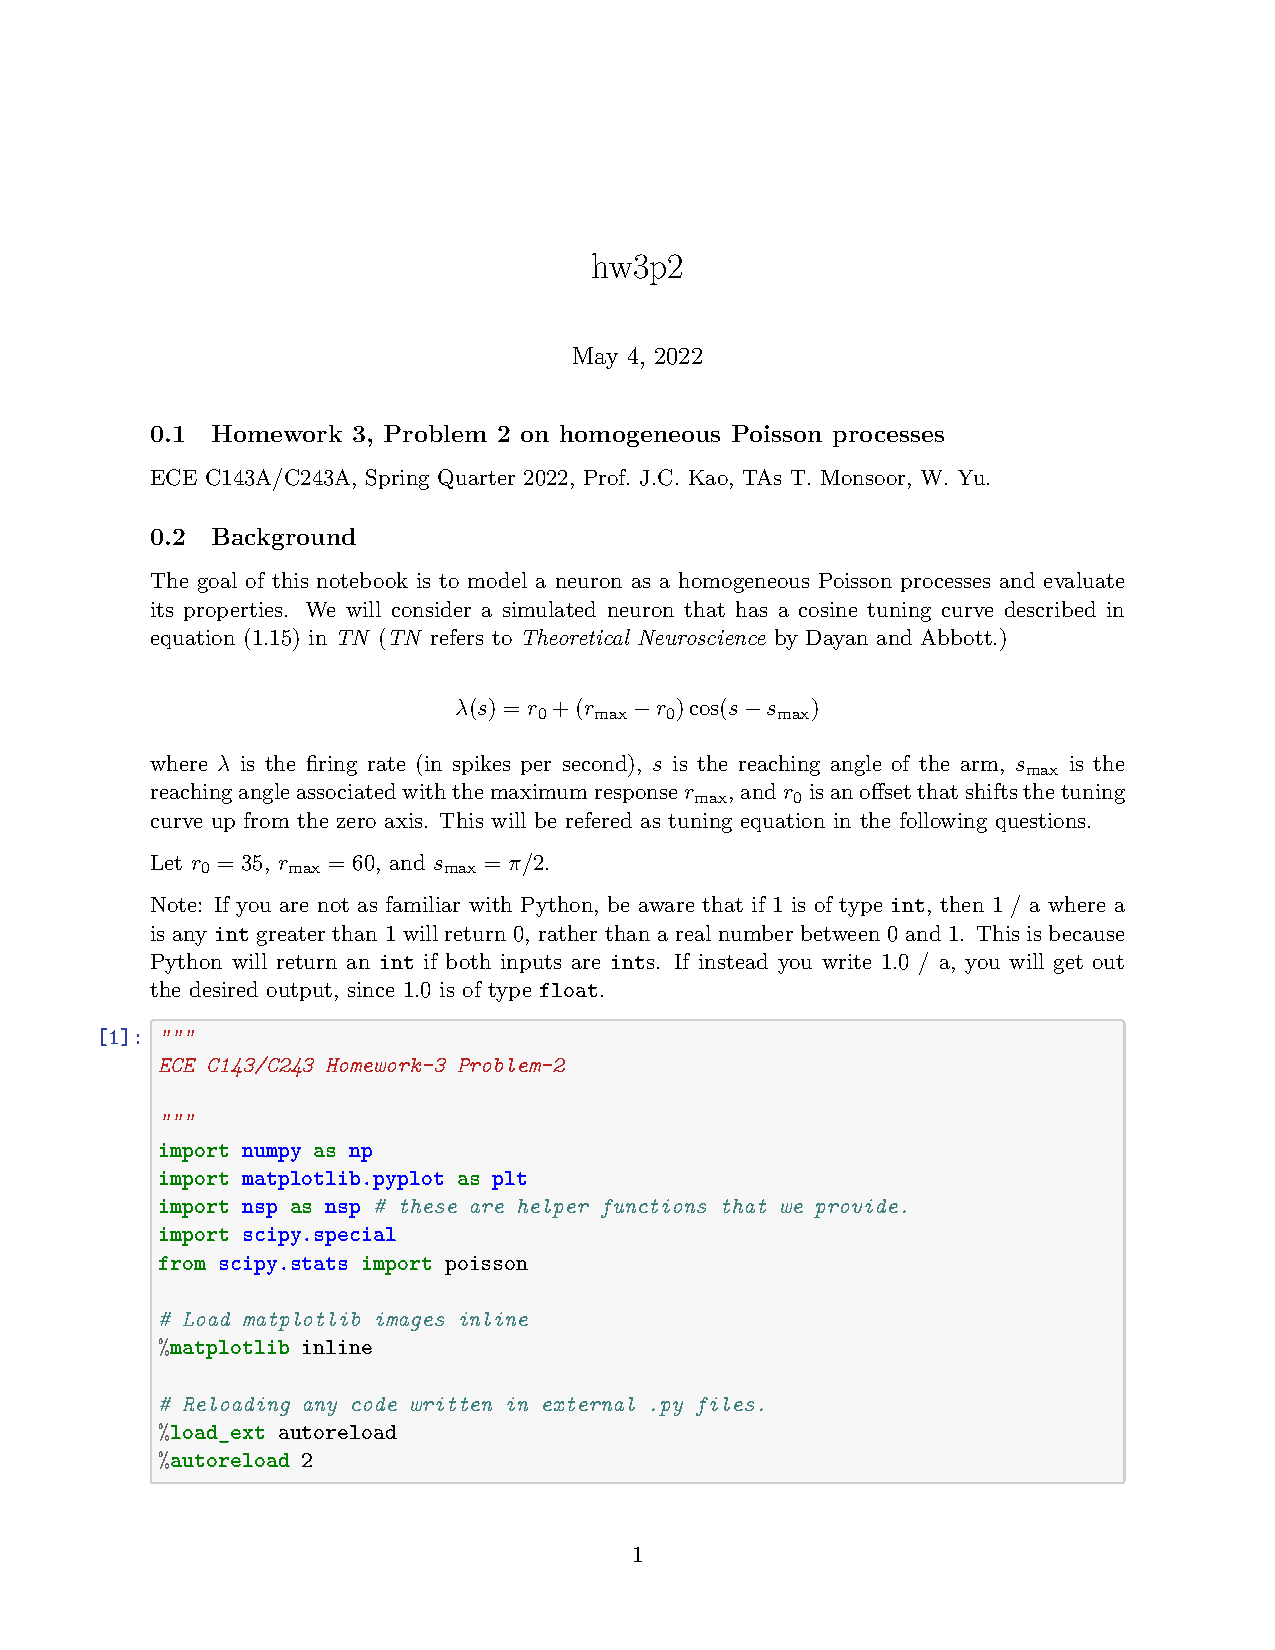
\includepdf[pages=-]{hw3p2.pdf}
%\section*{Problem 3}
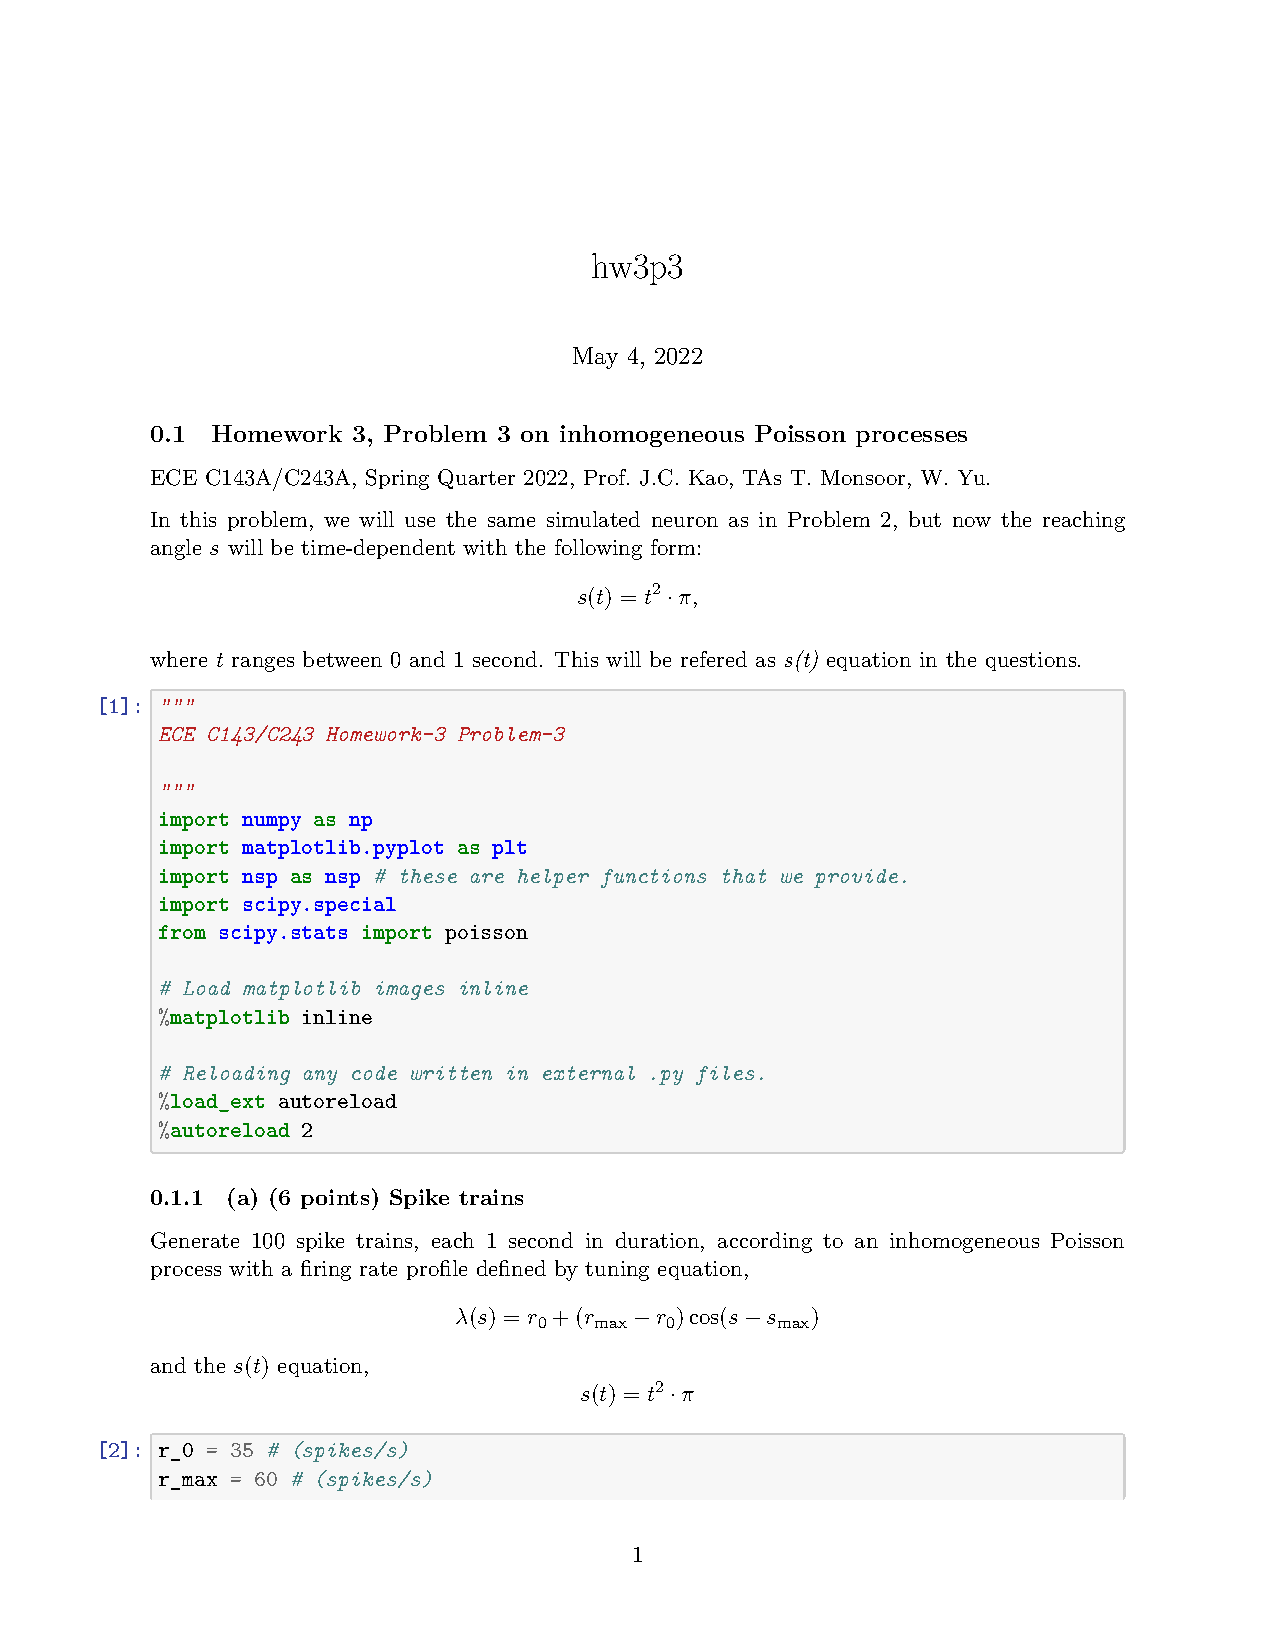
\includepdf[pages=-]{hw3p3.pdf}
%\section*{Problem 4}
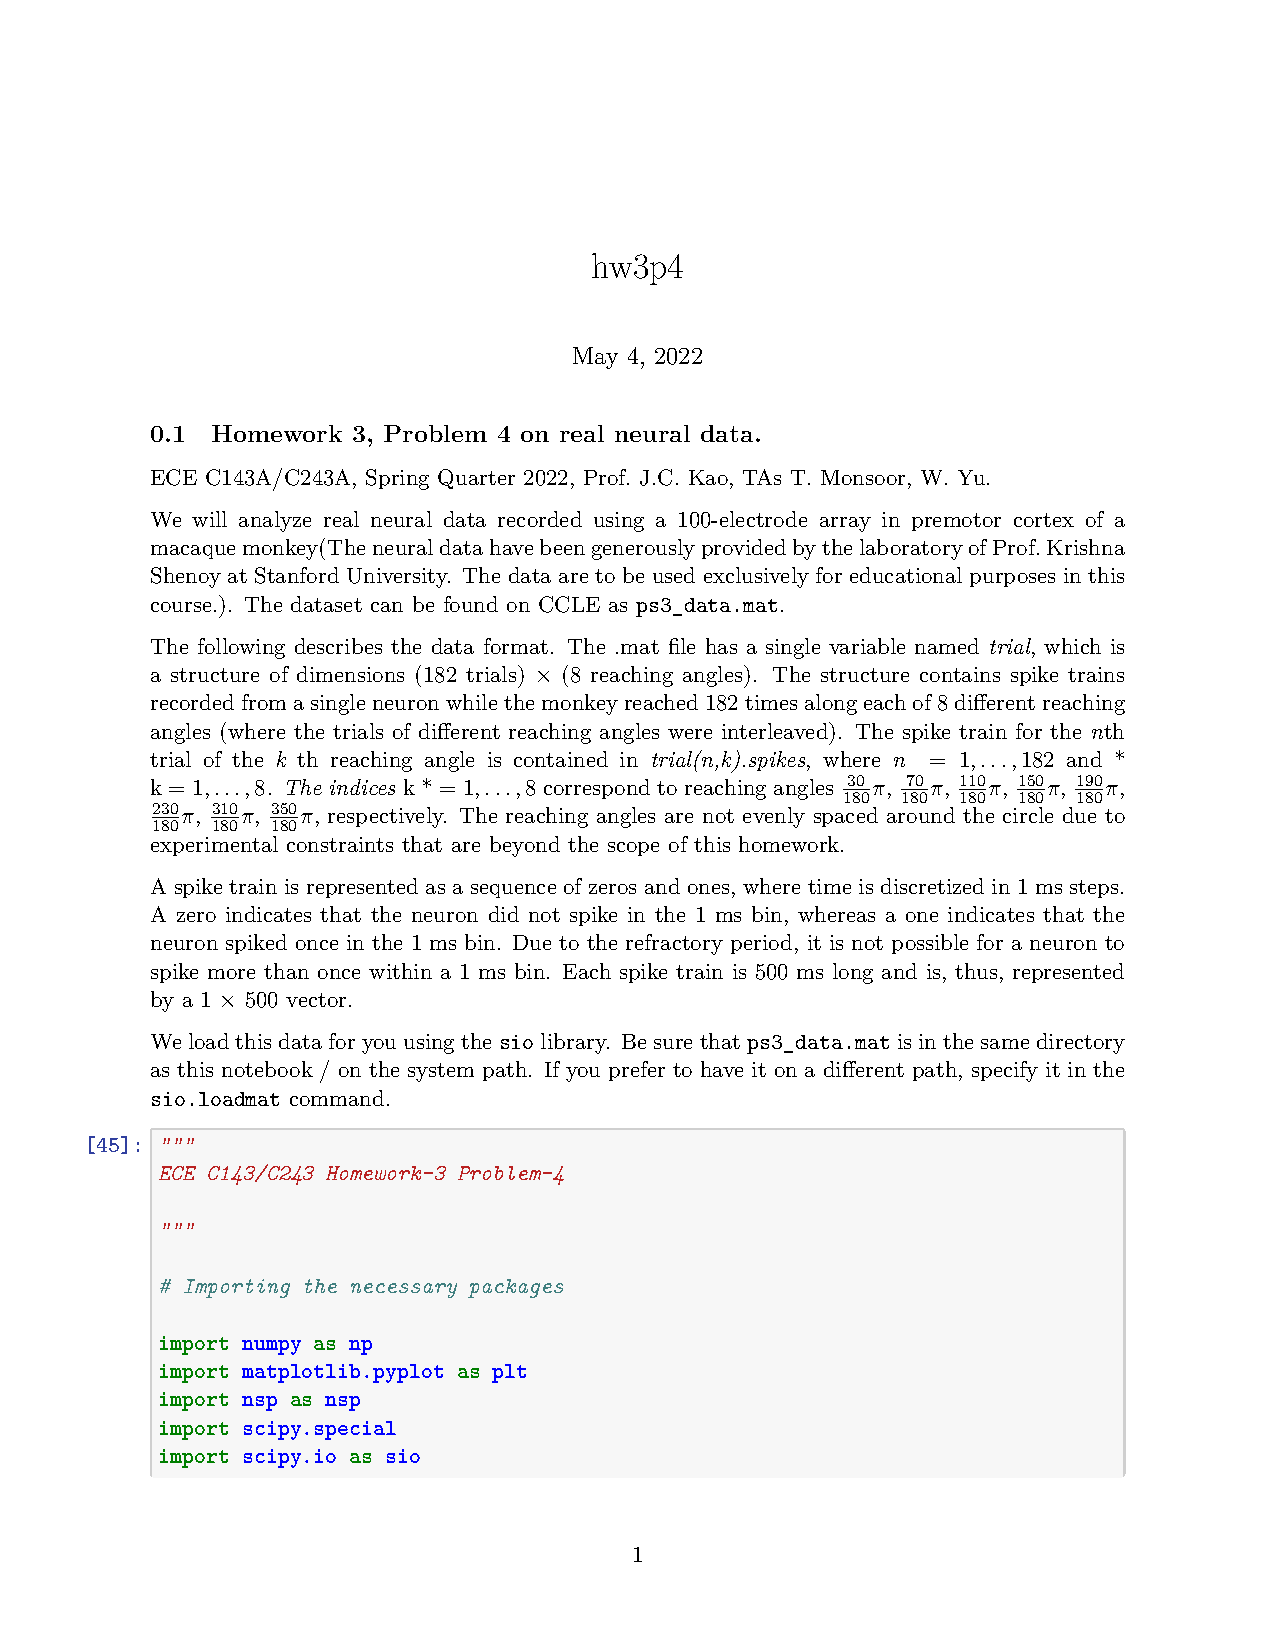
\includepdf[pages=-]{hw3p4.pdf}
\end{document}